\begin{exercise}
  Describe which tree on $V = [n]$  has the
  \begin{enumerate}
  \item Pr\"ufer code $(1,1,\dots,1)$.
  \item Pr\"ufer code $(1,2,3,\dots, n-2)$.
  \item Pr\"ufer code $(3,4,5,\dots, n)$.
  \item Pr\"ufer code $(n, n-1, n-2,\dots,4,3)$.
  \item Pr\"ufer code $(n-2,n-3,\dots,2,1)$.
  \item Pr\"ufer code $(1,2,1,2,\dots,1,2)$ (assuming $n$ is even).
 \end{enumerate}
 Justify and explain your answers.
\end{exercise}

\begin{figure}
\begin{center}
\caption{ }
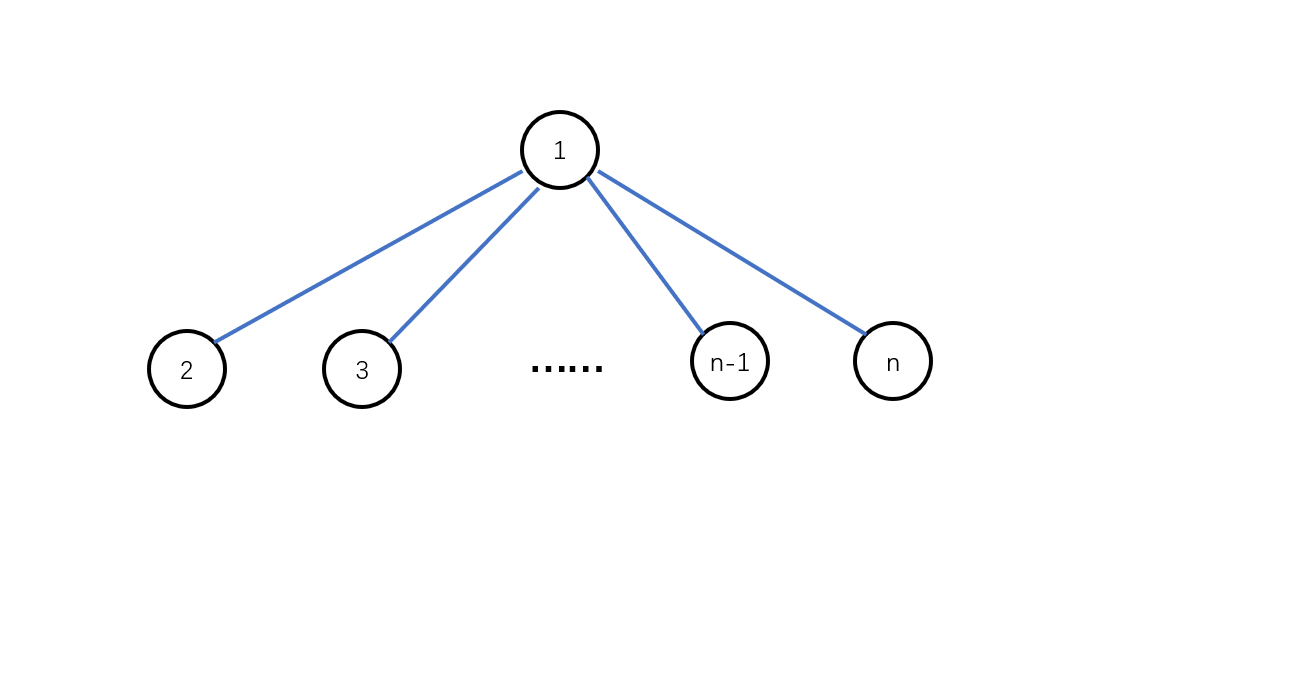
\includegraphics[scale=0.4]{figures/15_1.png}
\caption{ }
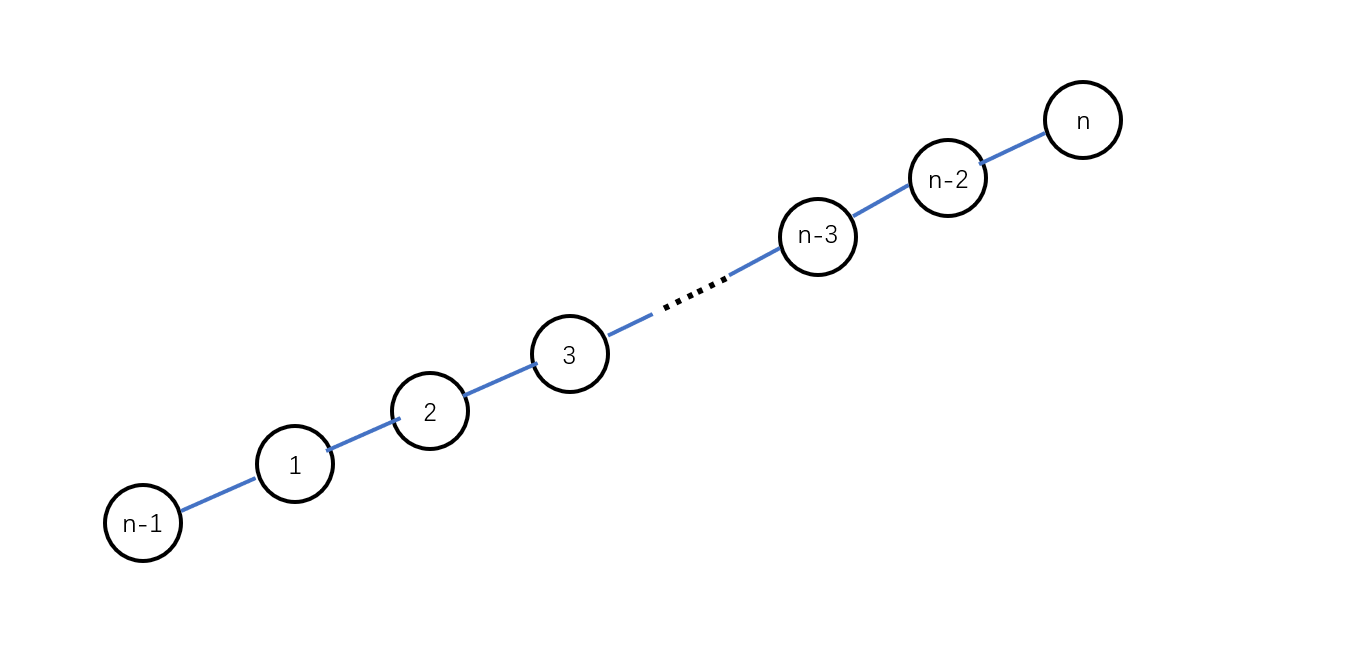
\includegraphics[scale=0.4]{figures/15_2.png}
\caption{ }
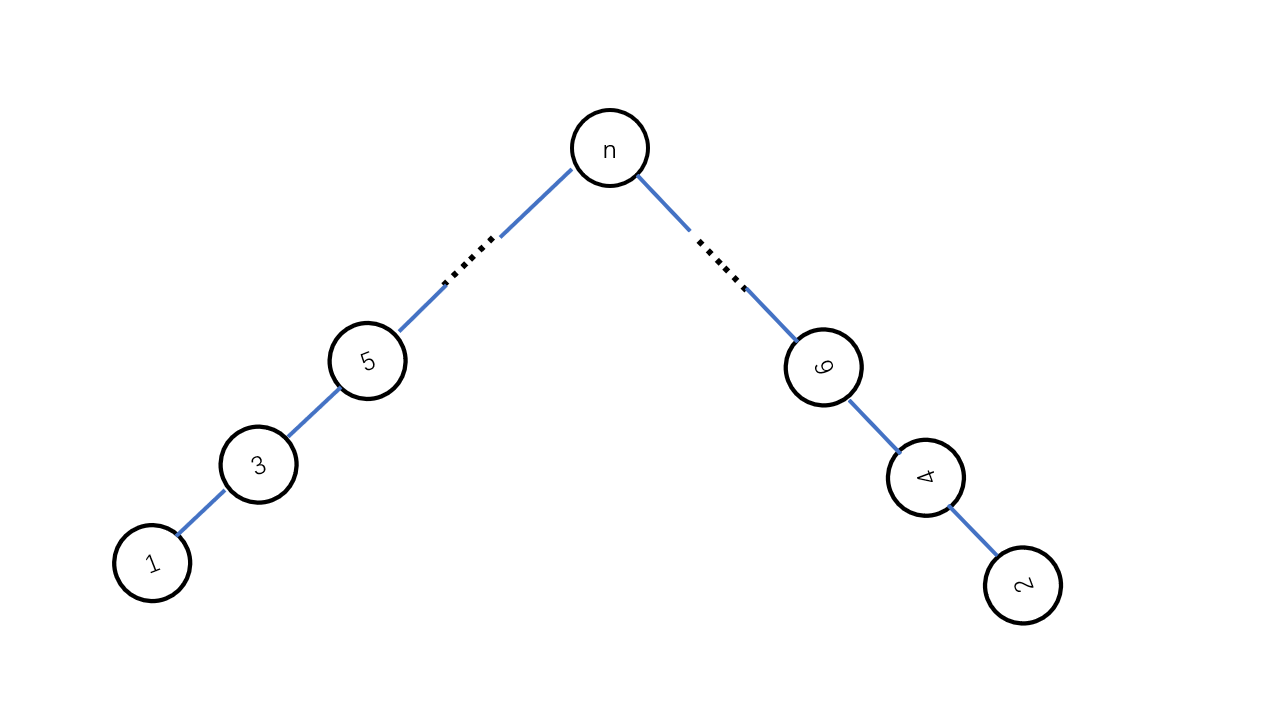
\includegraphics[scale=0.4]{figures/15_3.png}
\end{center}
\end{figure}
\begin{figure}
\begin{center}
\caption{ }
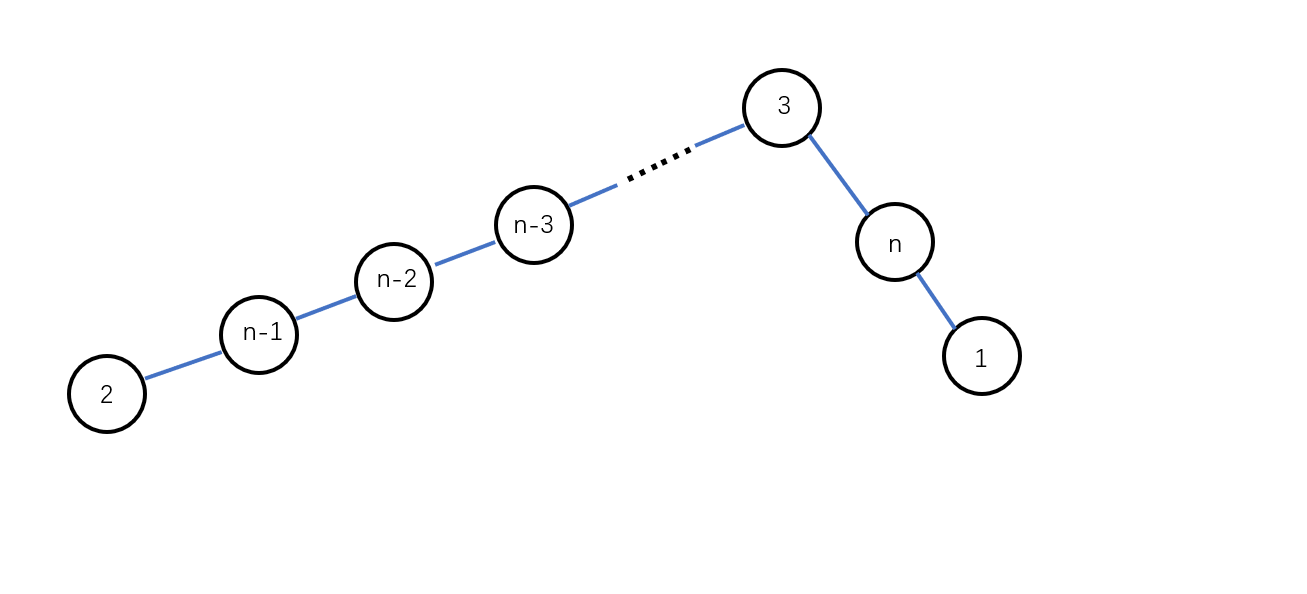
\includegraphics[scale=0.4]{figures/15_4.png}
\caption{ }
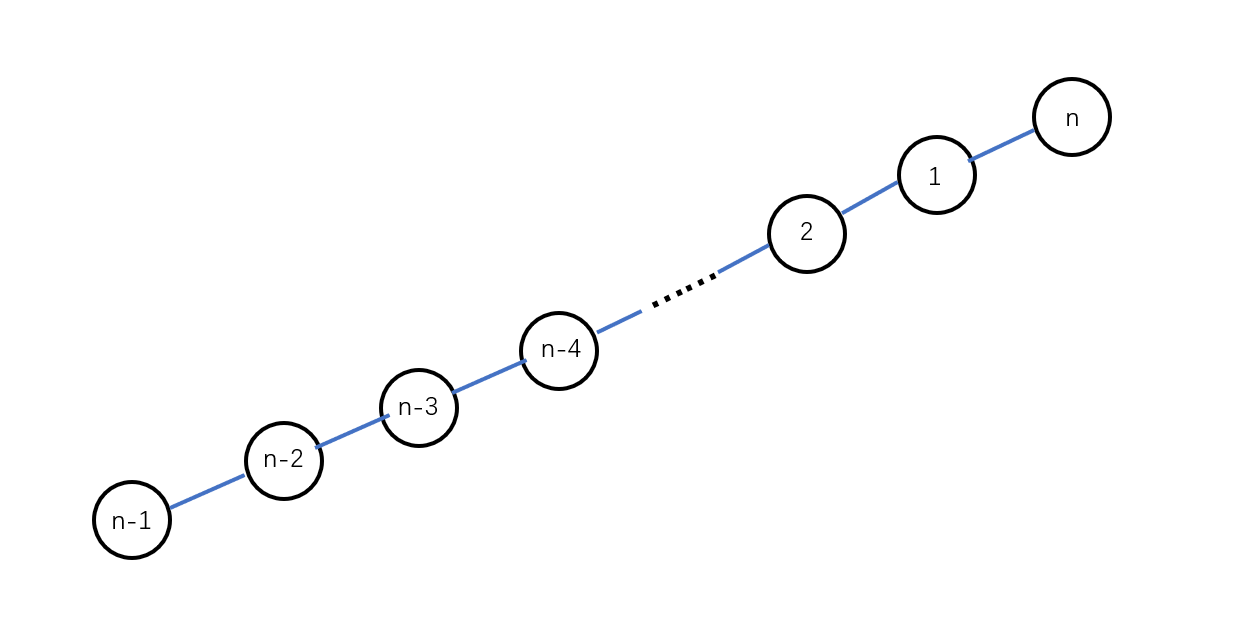
\includegraphics[scale=0.4]{figures/15_5.png}
\caption{ }
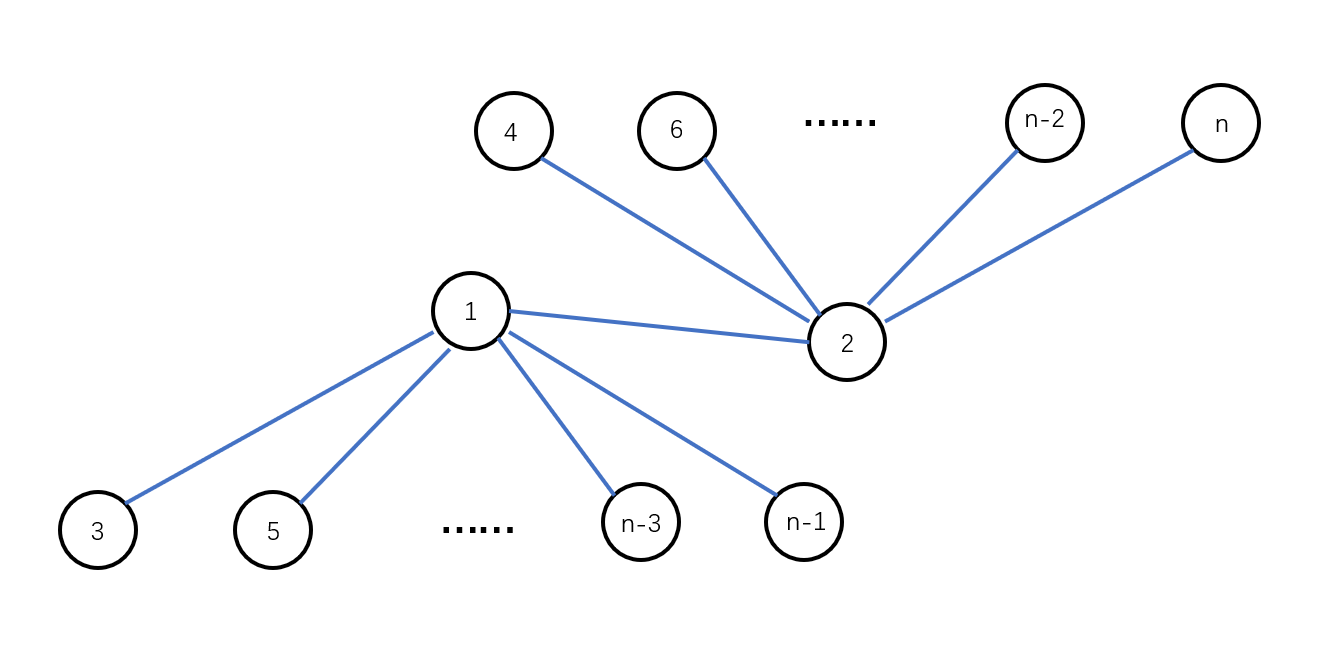
\includegraphics[scale=0.4]{figures/15_6.png}
\end{center}
\end{figure}
\begin{proof}
According to the algorithm to generate Pr\"ufer code:\\
1. Figure1: Cut the leaf 2,3,4\dots n-1 in turn, and so it's Pr\"ufer code is $(1,1,\dots,1)$.\\
2. Figure2: Cut the leaf n-1,1,2,3,4\dots n-3 in turn, and so it's Pr\"ufer code is $(1,2,3,\dots, n-2)$.\\
3. Figure3: Cut the leaf 1,2,3\dots n-2 in turn, and so it's Pr\"ufer code is $(3,4,5,\dots, n)$.\\
4. Figure4: Cut the leaf 1,2,n-1,n-2,n-3,\dots 4 in turn, and so it's Pr\"ufer code is $(n, n-1, n-2,\dots,4,3)$.\\
5. Figure5: Cut the leaf n-1,n-2,n-3,\dots 2 in turn, and so it's Pr\"ufer code is $(n-2,n-3,\dots,2,1)$.\\
6. Figure6: Cut the leaf 3,4,5,\dots ,n-1,1 in turn, and so it's Pr\"ufer code is $(1,2,1,2,\dots,1,2)$.\\
\end{proof}